\PassOptionsToPackage{table}{xcolor}
%hints from following:
%https://tex.stackexchange.com/questions/631549/passing-table-option-to-bespoke-class-not-recognised-by-xcolor
\documentclass{beamer}
\usepackage{ctex, hyperref}
\usepackage[T1]{fontenc}
\usepackage{sgamex}

% other packages
\usepackage{latexsym,amsmath,multicol,booktabs,calligra,xparse,hhline,array,multirow}
\usepackage{graphicx,pstricks,listings,stackengine,newtxtext,newtxmath,tikz,caption,subcaption,pgfplots,wasysym}



\author{赵万春}
\title{策略博弈}
\subtitle{findingnothing视频学习笔记}
\institute{天津财经大学 金融学院}
\date{2024年6月}
\usepackage{tufe}


% defs
\def\cmd#1{\texttt{\color{red}\footnotesize $\backslash$#1}}
\def\env#1{\texttt{\color{blue}\footnotesize #1}}
\definecolor{deepblue}{rgb}{0,0,0.5}
\definecolor{deepred}{rgb}{0.6,0,0}
\definecolor{deepgreen}{rgb}{0,0.5,0}
\definecolor{halfgray}{gray}{0.55}

\lstset{
	basicstyle=\ttfamily\small,
	keywordstyle=\bfseries\color{deepblue},
	emphstyle=\ttfamily\color{deepred},    % Custom highlighting style
	stringstyle=\color{deepgreen},
	numbers=left,
	numberstyle=\small\color{halfgray},
	rulesepcolor=\color{red!20!green!20!blue!20},
	frame=shadowbox,
}
\usefonttheme[onlymath]{serif}
%\pgfplotsset{compat=1.17}

	%for sgamex package：
	%One small inconvenience remains: because of a clash between the
	%hhline and beamer packages, if you are using sgamex with beamer you need
	%to add the following lines just before \begin{document}:
		\makeatletter
		\let\zz\reset@color
		\def\reset@color{\kern\z@\zz}
		\makeatother

\begin{document}

	\fangsong
\begin{frame}
	\titlepage
	\begin{figure}[htpb]
		\begin{center}
			
\includegraphics[width=0.2\linewidth]{pic/TJUFE_logo.png}
		\end{center}
	\end{figure}
\end{frame}	


\section{同时博弈与纳什均衡}

\subsection{同时行动博弈（策略性博弈）}

\begin{frame}[label = strategicgames]
	\frametitle{同时行动博弈（Strategic games）}
	不同的决策者同时选择行动方案并采取行动\\
	一个策略型博弈包括以下内容
	\begin{itemize}
		\item[$N$] 参与人
		\item[$A_{i}$] 参与人$i\in N$的行动集合
		\item[$\succsim_{i}$] 参与人$i$对博弈结果（行动组合）$\bigotimes_{j\in N} A_{j}$的偏好关系
		\item[$ u_{i} $] $\bigotimes_{j\in N} A_{j}\to \mathbb{R}$，用来表示偏好关系$\succsim_{i}$的效用函数
	\end{itemize}
	因此，同时行动博弈可以表示为：$\left\langle \overset{\text{参与人}}{N},\overset{\text{参与人能采取的行动}}{\left(A_{i}\right)},\overset{\text{采取行动的效用} }{\left(u_{i}\right)}\right\rangle$
	
\end{frame}
\begin{frame}[label = The Prisoner's Dilemma]
	\frametitle{例子：囚徒困境}

	\begin{center}
		\begin{game}{2}{2}[Player~1][Player~2]
			& $Defend$     & $Confess$\\
			$Defend$   & $3,3$  & $0,\alert{4}$\\
			$Confess$   & $\alert{4},0$   & $\alert{1},\alert{1}$
		\end{game}%\hspace*{\fill}
	\end{center}
	一般而言，方框左侧是参与人1的效用，方框右侧是参与人2的效用。\\
	存在严格占优均衡$ \left(Confess,Confess \right)$：无论对方选择$Defend$还是$Confess$，都是选择$Confess$更优。\\
	注意到，$\left(1,1\right)$并不是帕累托有效的。
\end{frame}

\begin{frame}[label = hawk_dove]
	\frametitle{例子：鹰鸽博弈}
	Hawk-Dove
	\begin{center}
		\begin{game}{2}{2}[Player~1][Player~2]
			& $Dove$ & $Hawk$\\
			$Dove$ & $3,3$ & $\alert{1},\alert{4}$\\
			$Hawk$ & $\alert{4},\alert{1}$ & $0,0$
		\end{game}
	\end{center}
	最优行动完全取决于对方的行动。
\end{frame}

\begin{frame}[label = matching_pennies]
	\frametitle{例子：抛硬币}
	Matching Pennies
	\begin{center}
		\begin{game}{2}{2}[Player~1][Player~2]
			& $Head$ & $Tail$\\
			$Head$ & $\alert{1},-1$ & $-1,\alert{1}$\\
			$Tail$ & $-1,\alert{1}$ & $\alert{1},-1$
		\end{game}
	\end{center}
	此时不存在纯策略纳什均衡
\end{frame}
\begin{frame}[label = battle_of_sex]
	\frametitle{例子：性别战博弈}
	Battle of Sex
	\begin{center}
		\begin{game}{2}{2}[Player~1][Player~2]
			& $Ballet$ & $Football$\\
			$Ballet$ & $\alert{1},\alert{2}$ & $0,0$\\
			$Football$ & $0,0$ & $\alert{2},\alert{1}$
		\end{game}
	\end{center}
	与鹰鸽博弈相反：均衡是相同行动。
\end{frame}

\subsection{纳什均衡}

\begin{frame}[label = defination_NE]
	\frametitle{符号定义}
	\begin{itemize}
		\item[$N$] 参与人集合$\left\lbrace 1,2,\dots,n\right\rbrace$
		\item[$a$] 行动集合，$a\in \bigtimes_{j\in N} A_j,\ a=\left(a_{1},\dots,a_{n}\right)$\footnote{很多文章直接定义策略集合而非行动集合，可能是同样的表述，故对应的字母大多为S}
		\item[$a_{-i}$] 除了$i$其他参与人采取行动的集合$a_{-i}=\left(a_{1},\dots,a_{i-1},a_{i+1},\dots,a_{n}\right)$，$a=\left(a_{i},a_{-i}\right)$
	\end{itemize}
	定义最优反应对应	\footnote{\text{对应中的}$x$\text{可以返回一个集合，而不只是函数中的数。}}(best response correspondence)\\
	对于参与人$i$，给定其他人反应$a_{-i}$，\\
	最优反应对应$B_{i}\left\lbrace a_{i}\in A_{i}:\ \underset{u\left(a_{-i},a_{i}\right)\geq u\left(a_{-i},a_{i}^{'}\right)}{\left(a_{-i},a_{i}\right)\succsim\left(a_{-i},a_{i}^{'}\right)} ,\forall a_{i}^{'}\in A_{i}\right\rbrace $

\end{frame}
\begin{frame}{纳什均衡}

		对于每个参与人$i$，采取的行动组合$a_{i}^{*}$属于最优反应对应$B_{i}\left(a_{-i}^{*}\right)$的行动组合集合$a^{*}=\left(a_{1}^{*},\dots ,a_{n}^{*}\right)$。即
		$$a_{i}^{*}\in B_{i}\left(a_{-i}^{*}\right),\forall i\in N$$

\end{frame}
\begin{frame}{囚徒困境}
	\begin{center}
		\begin{game}{2}{2}[Player~1][Player~2]
			& $D$     & $C$\\
			$D$   & $3,3$  & $0,4$\\
			$C$   & $4,0$   & $1,1$
		\end{game}%\hspace*{\fill}
	\end{center}
行动组合$a^{*}= \begin{array}{cc}
	 \left(D,D\right)   & \left(D,C\right)  \\
	 \left(C,D\right)   & \left(C,C\right) 
\end{array}$\\
$(D,D)$是均衡吗？换言之，对于Player 1，采取$ D $是Player2采取$ D $时的最优反应吗？\\
Player 1采取$ C $的效用更高$(3<4)$，因此$D\notin B_{1}\left(D\right)$\\
$(D,C)$是均衡吗？Player2采取$ C $时，Player1应采取$C$，因此$D\notin B_{1}\left(C\right)$\\
$(C,D)$是均衡吗？Player2采取$ D $时，Player1应采取$C$，因此$C\in B_{1}\left(D\right)$\\
$(C,C)$是均衡吗？Player2采取$ C $时，Player1应采取$C$，因此$C\in B_{1}\left(C\right)$
\end{frame}

\begin{frame}{囚徒困境}
	\begin{center}
		\begin{game}{2}{2}[Player~1][Player~2]
			& $D$     & $C$\\
			$D$   & $3,3$  & $0,4$\\
			$C$   & $4,0$   & $1,1$
		\end{game}%\hspace*{\fill}
	\end{center}
	行动组合$a^{*}= \begin{array}{cc}
		\left(D,D\right)   & \left(D,C\right)  \\
		\left(C,D\right)   & \left(C,C\right) 
	\end{array}$\\~\\
	同理，讨论Player 2的最优反应。\\
	$(D,D)$是均衡吗？Player1采取$ D $时，Player2应采取$C$，因此$D\notin B_{2}\left(C\right)$\\
	$(D,C)$是均衡吗？Player1采取$ D $时，Player2应采取$C$，因此$C\in B_{2}\left(C\right)$\\
	$(C,D)$是均衡吗？Player1采取$ C $时，Player2应采取$C$，因此$D\notin B_{2}\left(D\right)$\\
	$(C,C)$是均衡吗？Player1采取$ C $时，Player2应采取$C$，因此$C\in B_{2}\left(C\right)$
\end{frame}
\begin{frame}{囚徒困境}
	\begin{center}
		\begin{game}{2}{2}[Player~1][Player~2]
			& $D$     & $C$\\
			$D$   & $3,3$  & $0,4$\\
			$C$   & $4,0$   & $1,1$
		\end{game}%\hspace*{\fill}
	\end{center}
	行动组合$a^{*}= \begin{array}{cc}
		\left(D,D\right)   & \left(D,C\right)  \\
		\left(C,D\right)   & \left(C,C\right) 
	\end{array}$\\~\\
	总结\\
	因为$D\notin B_{1}\left(C\right)$,$D\notin B_{1}\left(C\right)$,$D\notin B_{2}\left(D\right)$，所以$(D,D)$、$(D,C)$、$(C,D)$都不是纳什均衡。\\
	只有$(C,C)$同时满足$C\in B_{2}\left(C\right)$和$C\in B_{1}\left(C\right)$，$(C,C)$是唯一纳什均衡。
\end{frame}

\begin{frame}{例子：鹰鸽博弈}
	Hawk-Dove
	\begin{center}
		\begin{game}{2}{2}[Player~1][Player~2]
			& $Dove$ & $Hawk$\\
			$Dove$ & $3,3$ & $1,4$\\
			$Hawk$ & $4,1$ & $0,0$
		\end{game}
	\end{center}
	同理，$H\in B_{1}\left(D\right)$，$D\in B_{1}\left(H\right)$，$H\in B_{2}\left(D\right),D\in B_{1}\left(H\right)$，因此$\left(D,H\right)$和$\left(H,D\right)$都是纳什均衡。\\
	先找best response，然后再确定是否互为best response。
\end{frame}

\begin{frame}{例子：抛硬币}
	Matching Pennies
	\begin{center}
		\begin{game}{2}{2}[Player~1][Player~2]
			& $Head$ & $Tail$\\
			$Head$ & $\alert{1},-1$ & $-1,\alert{1}$\\
			$Tail$ & $-1,\alert{1}$ & $\alert{1},-1$
		\end{game}
	\end{center}
\end{frame}

\section{纳什均衡的存在性：不动点定理}

\subsection{角谷不动点定理}

\begin{frame}[label = convex_and_compact]
	\frametitle{框架}
	讨论的内容都是$n$维欧式空间内($X\in\mathbb{R}$)，如果$X$是闭有界的，$X$为紧集。\\~\\
	集合$X$是凸的$\leftrightarrow \forall \alpha\in \left[0,1\right],\alpha x+\left(1-\alpha \right)y \in X$
	\begin{tikzpicture}
		% 画坐标轴
		\draw[->] (-1,0) -- (5,0) node[right] {$x$};
		\draw[->] (0,-1) -- (0,5) node[above] {$y$};
		
		% 画紧集（一个闭合的圆）
		\filldraw[fill=blue!20, draw=blue] (2,2) circle (1.5);
		
		% 标注紧集
		\node at (2,2) {紧集};
		
		% 画一些点
		\filldraw[fill=red] (1,1) circle (2pt);
		\filldraw[fill=red] (3,3) circle (2pt);
		\filldraw[fill=red] (2,3.5) circle (2pt);
		\filldraw[fill=red] (3.5,2) circle (2pt);
		
		% 标注点
		\node[below] at (1,1) {点A};
		\node[above] at (3,3) {点B};
		\node[above] at (2,3.5) {点C};
		\node[right] at (3.5,2) {点D};
	\end{tikzpicture}
\end{frame}
\begin{frame}[label = kakutani_fixed_point_theorem]
	\frametitle{角谷不动点定理}
	Kakutani's fixed point theorem\\~\\
	假定$X\in \mathbb{R}^{n}$是凸紧集，令$f:\ X\to X$为某个满足：\\
	(1)\ $\forall x\in X$，$f\left(x\right)$为非空的凸集\\
	(2)\ $f$的图像是闭的（$\forall$序列$\left\lbrace x_{n}\right\rbrace$和$\left\lbrace y_{n}\right\rbrace$，$\forall n$，$x_{n}\to x\left(\lim\limits_{n\to\infty} x_{n}=x\right)$，$y_{n}\to y$，$y_{n}\in f\left(x_{n}\right)$，有$y\in f\left(x\right)$。
	\\的映射，存在一个不动点$x^{*}$满足$x^{*}\in f\left(x^{*}\right)$
\end{frame}

\begin{frame}[label = kakutani_fixed_point_theorem_example]
	\frametitle{例子}
		\begin{center}
		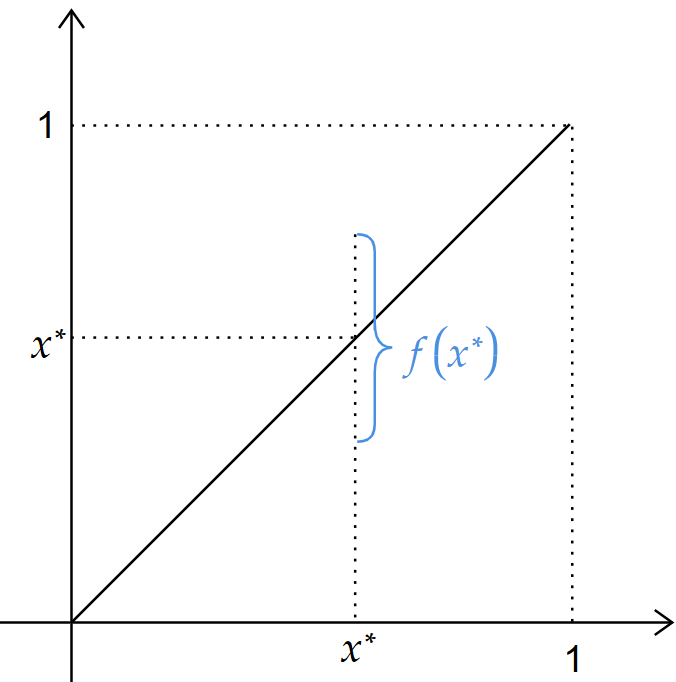
\includegraphics[width=0.5\linewidth]{pic/kakutani.png}
	\end{center}
\end{frame}

\begin{frame}[label = kakutani_not_hold]
	\frametitle{定理不成立？}
	1.不是紧集\\
	（1）不是闭集。$X=\left[0,1\right)$\\
	（2）无界。$X=\left[0,\infty\right)$\\
	2.不是凸集\\
	（1）断点。$X=\left[0,\frac{1}{3}\right]\cup\left[\frac{2}{3},1\right]$\\
	（2）开图象\\
	（3）对于某些$x$，$f\left(x\right)$非凸。\\
	（4）图象不满足对应条件
	\begin{center}
		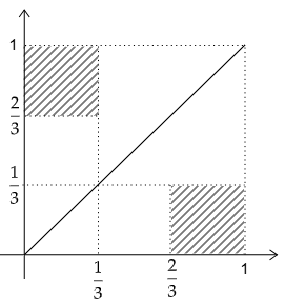
\includegraphics[width=0.3\linewidth]{pic/kakutanip1.png}
	\end{center}
\end{frame}

\subsection{纳什均衡的存在性}

\begin{frame}[label=continuousandquasiconcavepreference]
	\frametitle{偏好关系的连续性与拟凹性}
	定义偏好关系$\succsim$对于两个极限为$a$和$b$的收敛序列$\left\lbrace a^{k}\right\rbrace$和$\left\lbrace b^{k}\right\rbrace$，且$a^{k}\succsim b^{k}$，$a\succsim b$，则偏好关系$\succsim$\alert{是连续的}。\\
	定义欧式空间$\mathbb{R}^{n}$中的偏好关系$\succsim$满足对于任意$b\in \mathbb{R}^{n}$，集合$\underset{\text{上水平集}}{\left\lbrace a\in \mathbb{R}^{n}:\ a\succsim b\right\rbrace}$是凸集，则偏好关系$\succsim$\alert{是拟凹的}。\\~\\
\end{frame}

\begin{frame}[label=NEexist]
	\frametitle{纳什均衡的存在性}
	\begin{definition}[纳什均衡存在]
		\fangsong
		一个同时行动博弈$\left\langle N,\left(A_{i}\right),\left(z_{i}\right)\right\rangle$，对于所有的参与人$i\in N$满足:\\
		\begin{itemize}
			\item[1] $A_{i}\in \mathbb{R}$非空、凸集、紧集
			\item[2] 定义在$A_{i}\in \mathbb{R}$上的偏好关系$\succsim_{i}$连续、拟凹
		\end{itemize}
	\end{definition}

	根据偏好关系构建一个对应，才能使用kakutani不动点定理。\\
	偏好连续+拟凹=图象闭？
\end{frame}
\begin{frame}[label = best_response_correspondence]
	\frametitle{定义：最优反应对应}
	对于参与人$i$，给定其他人反应$a_{-i}$，最优反应对应$B_{i}\left(a_{-i}\right)=\left\lbrace a_{i}\in A_{i}:\ \underset{u\left(a_{-i},a_{i}\right)\geq u\left(a_{-i},a_{i}^{'}\right)}{\left(a_{-i},a_{i}\right)\succsim\left(a_{-1},a_{i}^{'}\right)} ,\forall a_{i}^{'}\in A_{i}\right\rbrace $\\
	在action profile上定义$B:A\to A$：action profile映射到最优反应对应的映射，即
	$$B\left(a\right)=\bigtimes\limits_{i\in N} B_{i}\left(a_{-i}\right)$$
	例如：
	$$B\left(\text{剪刀，石头}\right)=\{\left(\text{石头，布}\right)\}$$
	$$B\left(\text{剪刀，石头，布}\right)=\{\left(\text{布，剪刀，石头}\right)\}$$
	参与人1本来准备出剪刀，但参与人1在考虑到另外两个参与人会出石头和布后，参与人只有出布收益最高（一胜一平）。因此，右侧集合中参与人1的最优反应是布。\\
	换言之，$B$的文字表述是不用考虑参与人本来准备出什么，只需要考虑另外两个参与人的行动，再根据其他人反应得出最优反应。
\end{frame}

\begin{frame}[label = convexity_of_best_response_correspondence]
	\frametitle{证明：最优反应对应的凸性}
	注意到$A=\bigtimes\limits_{i\in N} A_{i}$是非空、紧集、凸集，只需证明对每个值都是凸的，图象是闭的。\\
	（偏好的拟凹性）\\
	$\forall i\in N, a_{-i}\in\bigtimes\limits_{j\in N\backslash\{i\}} A_{j}$，考虑任意$x,y\in B_{i}\left(a_{-i}\right)$，只需证\\
	$$\forall a_{i}^{'}\in A_{i} \left(a_{-i},x\right)\succsim_{i} \left(a_{-i},a_{i}^{'}\right)$$
	$$\forall a_{i}^{'}\in A_{i} \left(a_{-i},y\right)\succsim_{i} \left(a_{-i},a_{i}^{'}\right)$$
	(盯住一个outcome)\\
	注意到$\forall a_{i}^{'}\in A_{i}$，由偏好关系的拟凹性，$ \left\lbrace a\in \mathbb{R}^{n}:\ a\succsim_{i} \left(a_{-i},a_{i}^{'}\right)\right\rbrace $是凸的。
	取任意的$\alpha\in \left[0,1\right]$，由于$\alpha a_{-i}+\left(1-\alpha\right)a_{-i}=a_{-i}$\\
	构建凸组合$\left(\alpha_{-i},\alpha x+\left(1-\alpha\right)y\right)$，也满足$\left(\alpha_{-i},\alpha x+\left(1-\alpha\right)y\right)\succsim_{i}\left(a_{-i},a_{i}^{'}\right)$
	由$\left(\alpha_{-i},\alpha x+\left(1-\alpha\right)y\right)\in B_{i}\left(a_{-i}\right)$。因此对于所有$a\in A$，$B\left(a\right)$是凸的。
\end{frame}
\begin{frame}{证明拟凹性}
	考虑两个行动集合$\left\lbrace a^{k}\right\rbrace$和$\left\lbrace b^{k}\right\rbrace$，满足$b^{k}\in B\left(a^{k}\right)$，$a^{k}\in B\left(b^{k}\right)$以及$\lim\limits_{k\to\infty}a^{k}=a$，$\lim\limits_{k\to\infty}b^{k}=b$\\
	对于任意参与人$i\in N$，由最优反应对应定义，有$b^{k}_{i}\in B\left(a^{k}_{-i}\right)$\\
	即$\forall a_{i}^{'}\in A_{i}$，$\left(a_{-i}^{k},b_{i}^{k}\right)\succsim_{i}\left(a_{-i}^{k},a_{i}^{'}\right)$\\
	由偏好连续性，$\left(a_{-i},b_{i}\right)\succsim_{i}\left(a_{-i},a_{i}^{'}\right)$\\
	即$b_{i}\in B\left(a_{-i}\right)$，所以$b\in B\left(a\right)$\\~\\
	其实使用Tadelis证明2$\times $2博弈的框架更容易理解，不过放到后面混合博弈再谈。\\
	而且上面的纯策略例子中，由于option是离散的，所以并不满足convexity。
\end{frame}

\subsection{纳什均衡的意义}
\begin{frame}[label = implication_NE]
	\frametitle{纳什均衡的意义}
	“通俗地说，在一个纳什均衡中，对于每个参与人来说，给定其他人的行动，这个人的行动是其他人行动的一个最优反应。”\\
	在假设每个参与人都是理性的情况下可以预测的结果（囚徒困境）\\
	但如果包含多个纳什均衡，预测性会不成立（性别博弈）\\
	焦点（选牌）\\
	自我约束：implementation\\
	稳态（卷、靠右走）
\end{frame}

\subsection{零和博弈}
\begin{frame}{零和？}
	\begin{center}
		\begin{game}{2}{2}[Player~1][Player~2]
			& $Head$ & $Tail$\\
			$Head$ & $\alert{1},-1$ & $-1,\alert{1}$\\
			$Tail$ & $-1,\alert{1}$ & $\alert{1},-1$
		\end{game}
	\end{center}
	\begin{center}
		\begin{game}{3}{3}[Player~1][Player~2]
			& $L$ & $M$ & $R$\\
			$H$ & $2,-2$ & $\alert{0},\alert{0}$ & $1,-1$\\
			$M$ & $\alert{4},-4$ & $-3,\alert{3}$ & $\alert{2},-2$\\
			$D$ & $1,-1$ & $-2,\alert{2}$ & $-2,\alert{2}$
		\end{game}
	\end{center}
	对于有两个参与人$\{1,2\}$的零和博弈$\left\langle \{1,2\} , \left(A_{i}\right) , \left(u_{i}\right)\right\rangle$，满足$u_{1}+u_{2}=0$。\\
\end{frame}

\begin{frame}{\fangsong{最大——最小策略}}
	首先假定对方一定会最小化自己的收益，然后再选择最大化自己收益的策略。\\
	定义：最大最小策略(maxminimizer)
	如果行动$x^{*}\in A_{1}$是博弈$\left\langle \{1,2\} , \left(A_{i}\right) , \left(u_{i}\right)\right\rangle$中参与人1的最大——最小策略，有
	$$\forall x^{*}\in A_{1} ,\min_{y\in A_{2}}u_{1}\left(x^{*},y\right)\geq\min_{y\in A_{2}} u_{1}\left(x,y\right)$$
	参与人1先选择了自己的收益$x^{*}$，然后参与人2采取了使参与人1收益最小的策略$y$。\\
	即在假定自己的收益会被对方最小化的前提下，保证获取最大的收益，但并没有先后。同理，
	$$\forall y^{*}\in A_{2} ,\min_{x\in A_{1}}u_{2}\left(x,y^{*}\right)\geq\min_{x\in A_{1}} u_{2}\left(x,y\right)$$
\end{frame}

\begin{frame}{例子：matching pennis}
	最大——最小策略用斜体表示，即参与人1在做出选择后，参与人2最小化参与人1收益的选择。\\
	无论head或者tail都是最大——最小策略。
	\begin{center}
		\begin{game}{2}{2}[Player~1][Player~2]
			& $Head$ & $Tail$\\
			$Head$ & $\alert{1},-1$ & $\textit{-1},\alert{1}$\\
			$Tail$ & $\textit{-1},\alert{1}$ & $\alert{1},-1$
		\end{game}
	\end{center}
\end{frame}
\begin{frame}{例子}
	首先，参与人2最小化参与人1在对应选项下的收益
	\begin{center}
		\begin{game}{3}{3}[Player~1][Player~2]
			& $L$ & $M$ & $R$\\
			$\alert{\rightarrow }H$ & $2,-2$ & $\textit{\alert{0}},\alert{0}$ & $1,-1$\\
			$M$ & $\alert{4},-4$ & $\textit{-3},\alert{3}$ & $\alert{2},-2$\\
			$D$ & $1,-1$ & $\textit{-2},\alert{2}$ & $\textit{-2},\alert{2}$
		\end{game}
	\end{center}
	然后参与人1再对比这些收益（斜体）哪个更高，做出选择。
\end{frame}
\begin{frame}{例子}
	然后，参与人1最小化参与人2在对应选项下的收益
	\begin{center}
		\begin{game}{3}{3}[Player~1][Player~2]
			& &$\downarrow$&\\
			& $L$ & $M$ & $R$\\
			$H$ & $2,-2$ & $\alert{0},\textit{\alert{0}}$ & $1,-1$ \\
			$M$ & $\alert{4},\textit{-4}$ & $-3,\alert{3}$ & $\alert{2},\textit{-2}$\\
			$D$ & $1,-1$ & $-2,\alert{2}$ & $-2,\alert{2}$
		\end{game}
	\end{center}
	然后参与人2再对比这些收益（斜体）哪个更高，做出选择。
\end{frame}

\begin{frame}{零和博弈纳什均衡与最大最小策略}
	命题：考虑零和博弈$\left\langle \{1,2\} , \left(A_{i}\right) , \left(u_{i}\right)\right\rangle$，若$\left(x^{*},y^{*}\right)$为其一个纳什均衡，参与人1的一个最大——最小策略是$x^{*}$，参与人2的一个最大最小策略是$y^{*}$。\\
	在考虑最大——最小策略时，参与人把对方当成了nature的一部分。\\
	证明：
	若$\left(x^{*},y^{*}\right)$为零和博弈的纳什均衡，\\
	根据纳什均衡的定义，对于任意$y\in A_{2}$，有$u_{2}\left(x^{*},y^{*}\right)\geq u_{2}\left(x^{*},y^{*}\right)$\\
	注意到$u_{2}=-u_{1}$，即对于任意$y\in A_{2}$，$-u_{1}\left(x^{*},y^{*}\right)\geq -u_{1}\left(x^{*},y^{*}\right)$\\
	去掉负号，即
	$$u_{1}\left(x^{*},y^{*}\right)\leq u_{1}\left(x^{*},y^{*}\right)$$
	$$u_{1}\left(x^{*},y^{*}\right)\leq \min_{y\in A_{2}} u_{1}\left(x^{*},y\right)\leq \max_{x\in A_{1}}\min_{y\in A_{2}} u_{1}\left(x,y\right)$$
	反向同理，可得
	$$u_{1}\left(x^{*},y^{*}\right)\geq \max_{x\in A_{1}}\min_{y\in A_{2}} u_{1}\left(x,y\right)$$
	即
	$$u_{1}\left(x^{*},y^{*}\right) = \max_{x\in A_{1}}\min_{y\in A_{2}} u_{1}\left(x,y\right),u_{2}\left(x^{*},y^{*}\right) = \max_{y\in A_{2}}\min_{x\in A_{1}} u_{2}\left(x,y\right)$$
\end{frame}

\section{混合策略纳什均衡}
\subsection{混合策略纳什均衡}
\begin{frame}[label = MNE_definition]
	\frametitle{混合策略纳什均衡的定义}
	对于策略博弈$G=\left\langle N, \left(A_{i}\right) ,\left(u_{i}\right)\right\rangle$，$A_{i}=\left\lbrace a_{1},...,a_{m} \right\rbrace$\\
	采取$A_{i}$中行动的概率$$\Delta\left(A_{i}\right)\left\lbrace \left(p_{1},...,p_{m}\right)\in \mathbb{R}^m_{+} \middle| \sum_{i=1}^{m} p_{i} =1 	\right\rbrace\footnote{单纯形。把概率赋予到$ A_{i} $}$$
	定义参与人$ i $的混合策略$\alpha_{i}\in \Delta\left(A_{i}\right)$，混合策略集合$\alpha
	=\left(\alpha_{1},\alpha_{2},...,\alpha_{|N|}\right)\in \bigtimes\limits_{j\in N} \Delta\left(A_{j}\right)$\\
	定义VNM效用$u_{i}:\bigtimes\limits_{j\in N} \Delta\left(A_{j}\right)\to \mathbb{R}$，满足
	$$U_{i}\left(\alpha\right)=\sum_{a\in A}\left(\prod_{j\in N} \alpha_{j}\left(a_{j}\right)\right)u_{i}\left(a\right)
	\footnote{$a$这一结果发生的概率，是由第$j$个人采取$a_{j}$策略的概率$\alpha_{j}$决定的，必须每个$j$都各自采取实现$a$这一结果的概率.在此基础上加总，即所有结果依概率产生的全部outcome}$$
	同时行动博弈$G=\left\langle N, \left(A_{i}\right) ,\left(u_{i}\right)\right\rangle$的混合扩展表示为$\left\langle N, \left(\Delta\left(A_{i}\right)\right) ,\left(U_{i}\right)\right\rangle$
\end{frame}
\begin{frame}[label = MNE_definition_example]
	\frametitle{MNE的例子：剪刀石头布}
	考虑剪刀石头布$\left\langle \left\lbrace 1,2\right\rbrace, \left(\left\lbrace\text{剪刀，石头，布}\right\rbrace\right),\left(u_{i}\right) \right\rangle$\\
	假定$\alpha_{1}=\left(\frac{1}{3},\frac{1}{3},\frac{1}{3}\right),\alpha_{2}=\left(\frac{1}{2},\frac{1}{2},0\right)$\\
	$$U_{1}\left(a_{1},a_{2}\right)=
	\frac{1}{3}\times\frac{1}{2}\times u_{1}\left(\text{剪刀，石头}\right)
	+\frac{1}{3}\times\frac{1}{2}\times u_{1}\left(\text{石头，剪刀}\right)$$
	$$+\frac{1}{3}\times\frac{1}{2}\times u_{1}\left(\text{布，剪刀}\right)
	+\frac{1}{3}\times\frac{1}{2}\times u_{1}\left(\text{布，石头}\right)
	\footnote{去掉了$u_{1}=u_{2}=0$和出布的结果}$$
	$$=\frac{1}{3}\times\frac{1}{2}\times\left(-1+1-1+1\right)=0$$
\end{frame}


\begin{frame}[label = MNE_and_expansion]
	\frametitle{由Matching Pennies解释混合扩张}
	同时行动博弈的混合策略纳什均衡等价于\textbf{同时行动博弈混合扩张}\footnote{已经不是同一个game了}的纳什均衡。\\
	\begin{center}
		\begin{game}{2}{2}[Player~1][Player~2]
			& $Head$ & $Tail$\\
			$Head$ & $\alert{1},-1$ & $-1,\alert{1}$\\
			$Tail$ & $-1,\alert{1}$ & $\alert{1},-1$
		\end{game}
	\end{center}
	假定$\alpha_{1}=\left(p,1-p\right)$，$\alpha_{2}=\left(q,1-q\right)$\\
	参与人1的payoff:
	\begin{align}
		Head :& q\times 1 + \left(1-q\right)\times \left(-1\right)=2q-1&\\
		Tail :& q\times \left(-1\right) + \left(1-q\right)\times 1=1-2q&
	\end{align}


\end{frame}

\begin{frame}[label = mixed_expansion_best_respond_correspondence]
	\frametitle{混合扩张的最优反应对应}
		若$2q-1>1-2q$，即$q>\frac{1}{2}$，参与人1的最优反应对应$B_{1}\left(\alpha_{2}\right)$满足
	\begin{equation}
		B_{1}\left(\alpha_{2}\right)=\left\lbrace
		\begin{aligned}
			&\lbrace\left(1,0\right)\rbrace & , \ if \ q > \frac{1}{2}\\
			&\lbrace\left(p,1-p\right)|0 \leq p\leq 1\rbrace & , \ if \ q = \frac{1}{2}\\
			&\lbrace\left(0,1\right)\rbrace & , \ if \ q < \frac{1}{2}
		\end{aligned}
		\right.
	\end{equation}
	同理，
	\begin{equation}
		B_{2}\left(\alpha_{1}\right)=\left\lbrace
		\begin{aligned}
			&\lbrace\left(1,0\right)\rbrace  ,& \ if \ p < \frac{1}{2}\\
			&\lbrace\left(q,1-q\right)|0 \leq q\leq 1\rbrace  ,& \ if \ p = \frac{1}{2}\\
			&\lbrace\left(0,1\right)\rbrace  ,& \ if \ p > \frac{1}{2}
		\end{aligned}
		\right.
	\end{equation}
\end{frame}

\begin{frame}[label = how_to_find_MNE1]
	\frametitle{如何找MNE？}
	\begin{center}
		\begin{tikzpicture}
			% 绘制 x 轴
			\draw[->] (0,0) -- (5.2,0) node[right] {$p$};
			% 绘制 y 轴
			\draw[->] (0,0) -- (0,5.2) node[above] {$q$};
			% 绘制红色区域
			\draw[red, line width=1.0] (0,5) -- (2.5,5) -- (2.5,0) -- (5,0);
			% 标注 Player2 的最优反应
			\node[red, above] at (2.5,5) {Player2的最优反应};
			% 标注其他点
			\node[left] at (0,5) {$1$};
			\node[left] at (0,2.5) {$\frac{1}{2}$};
			\node[below] at (2.5,0) {$\frac{1}{2}$};
			\node[below] at (5,0) {$1$};
		\end{tikzpicture}
	\end{center}
\end{frame}
\begin{frame}[label = how_to_find_MNE2]{如何找MNE？}
	\begin{center}
		\begin{tikzpicture}
			% 绘制 x 轴
			\draw[->] (0,0) -- (5.2,0) node[right] {$p$};
			% 绘制 y 轴
			\draw[->] (0,0) -- (0,5.2) node[above] {$q$};
			% 绘制红色区域
			\draw[red, line width=1.0] (0,5) -- (2.5,5) -- (2.5,0) -- (5,0);
			% 标注 Player2 的最优反应
			\node[red, above] at (2.5,5) {Player2的最优反应};
			% 绘制蓝色区域
			\draw[blue, line width=1.0] (0,0) -- (0,2.5) -- (5,2.5) -- (5,5);
			% 标注 Player1 的最优反应
			\node[blue, right] at (5,2.5) {Player1的最优反应};
			% 标注其他点
			\node[left] at (0,5) {$1$};
			\node[left] at (0,2.5) {$\frac{1}{2}$};
			\node[below] at (2.5,0) {$\frac{1}{2}$};
			\node[below] at (5,0) {$1$};
			% MNE
			\node[circle, fill=black, inner sep=2pt] at (2.5,2.5) {};
			\node[above right] at (2.5,2.5) {MNE} ;
		\end{tikzpicture}
	\end{center}
\end{frame}

\againframe{continuousandquasiconcavepreference}
\againframe{NEexist}

\begin{frame}[label = prove_MNE]
	\frametitle{同时行动博弈的MNE证明思路}
	同时行动博弈的MNE通过单纯形$\Delta \left(A\_{i}\right)$定义，相当于直接考虑凸包，自然是凸的\\
	集合有限，显然是非空紧集\\
	单纯形定义在欧式空间\\
	因此，只需要考虑偏好关系的连续性与拟凹性。
\end{frame}

\againframe{matching_pennies}

\begin{frame}[label = strategicgameMNEexist]
	\frametitle{同时行动博弈的MNE存在性}
	同时行动博弈的MNE通过单纯形$\Delta \left(A\_{i}\right)$定义，相当于直接考虑凸包，自然是凸的\\
	集合有限，显然是非空紧集\\
	单纯形定义在欧式空间\\
	因此，只需要考虑偏好关系的连续性与拟凹性。\\
	\begin{theorem}[策略博弈MNE存在性]
		\fangsong 
		任何有限策略博弈都具有混合策略纳什均衡。
	\end{theorem}
\end{frame}

\begin{frame}[label = MNE_Delta_A_i_close]
	\frametitle{证明：MNE的action profile单纯形$ \Delta \left(A_{i}\right) $为闭集}
	假设$G$是有穷的同时行动博弈，$\forall i \in N $，$A_{i}$是有穷的。令$A_{i}=\lbrace a_{1},a_{2},...,a_{m} \rbrace$，只需证明
	$$\Delta \left(A_{i}\right)=\left\lbrace\left(p_{1},p_{2},...,p_{m}\right)\in \left[0,1\right]^{m} \middle| \sum_{k=1}^{m} p_{k} = 1 \right\rbrace$$
	非空、欧氏空间的子集、紧集。\\
	为证明集合为闭集，考虑序列$\left\lbrace \left(p_{1}^{k},p_{2}^{k},...,p_{m}^{k}\right) \right\rbrace\subseteq \Delta\left(A_{i}\right)$，极限为$ \left(p_{1}^{*},p_{2}^{*},...,p_{m}^{*}\right) ,k\to \infty$\\
	由于$\left[0,1\right]$区间是闭的，对于$\lbrace p_{l}^{k} \rbrace \in \left[0,1\right]$，$\lim\limits_{k\to\infty}p_{l}^{k}\in \left[0,1\right]$\\
	由于$\sum\limits_{l=1}^{m} p_{l}^{k}=1$，	$\lim\limits_{k\to\infty}\sum\limits_{l=1}^{m} p_{l}^{k}=1$，有$\sum\limits_{l=1}^{m} p_{l}^{*}=1$，因此$ \left(p_{1}^{*},p_{2}^{*},...,p_{m}^{*}\right)\in\Delta \left(A_{i}\right) $。\\
	$ \Delta \left(A_{i}\right) $为闭集，证毕。
\end{frame}

\begin{frame}[label = MNE_Delta_A_i_convex]
	\frametitle{证明：凸性，即$ \Delta \left(A_{i}\right) $为凸，即证凸组合在$ \Delta \left(A_{i}\right) $中}
	考虑$\left(p_{1},p_{2},...,p_{m}\right),\left(q_{1},q_{2},...,q_{m}\right)\in \Delta \left(A_{i}\right)$\\
	对于$\forall \alpha \in \left[0,1\right],$，只需检验
	$$\alpha\left(p_{1},p_{2},...,p_{m}\right)+\left(1-\alpha\right)\left(q_{1},q_{2},...,q_{m}\right)\in \Delta \left(A_{i}\right)$$
	即检验
	$$\left( \alpha p_{1} + \left(1-\alpha\right) q_{1} ,\alpha p_{2} + \left(1-\alpha\right) q_{2} ,...,\alpha p_{m} + \left(1-\alpha\right) q_{m}\right)$$
	注意到对于任意$l\in \left\lbrace1,...,m \right\rbrace$，$p_{l},q_{l}\in \left[0,1\right]$，即$$\alpha p_{l}\in \left[0,\alpha\right],\left(1-\alpha\right) q_{l}\in \left[0,1-\alpha\right]$$
	有$\alpha p_{l} + \left(1-\alpha\right) q_{l} \in \left[0,1\right]$。\\
	然后证明所有的凸组合之和等于1.
	$$\sum_{l=1}^{m}\alpha p_{l}+\left(1-\alpha\right)q_{l}=\alpha \sum_{l=1}^{m}p_{l}+\left(1-\alpha\right)\sum_{l=1}^{m}q_{l}=1$$
\end{frame}
\begin{frame}[label = MNE_preference_continuous]
	\frametitle{证明：MNE偏好关系的连续性}
	\begin{theorem}[VNM效用函数的偏好关系]
		\fangsong 
		对于$a,b\in \Delta \left(\bigtimes\limits_{j\in N}A_{j}\right)$，$a\apprge b$当且仅当$U_{i}\left( a\right) \geqslant U_{i}\left( b\right) $
	\end{theorem}
	 注意到$U_{i}=\sum\limits_{a\in A}\left(\prod\limits_{j\in N} \alpha_{j}\left(a_{j}\right)\right)u_{i}\left(a\right)$为关于$\alpha$的线性函数，具有连续性。因此偏好关系$\apprge_{i}$对于任意$i$都是连续的。
\end{frame}

\begin{frame}[label = MNE_preference_quasi_concave]
	\frametitle{证明：MNE偏好关系的拟凹性}
	考虑偏好关系的上水平集$\left\lbrace a\in \mathbb{R}^{n}:\ a\succsim b\right\rbrace$：
	$$S=\left\lbrace a\in \mathbb{R}^{m} \middle| U_{i}\left(a\right) \geq U_{i}\left(b\right)\right\rbrace $$
	令$a_{1},a_{2}\in S , \alpha\in \left[0,1\right]$，\\

	\begin{equation}
		\begin{aligned}
			U_{i}\left( \alpha a_{1}+\left( 1-\alpha\right) a_{2}\right) &=\sum\limits_{a\in A}\left(\prod_{j\in N}\left(\alpha a_{1}+\left( 1-\alpha\right) a_{2}\right) \left(a_{j}\right)\right)u_{i}\left(a\right)\\
			&=\alpha \underbrace{\sum\limits_{a\in A}\prod\limits_{j\in N}a_{1}\left(a_{j}\right)u_{i}\left(a\right)}_{U_{i}\left(a\right)}+ \left(1-\alpha\right) \underbrace{\sum\limits_{a\in A}\prod\limits_{j\in N}a_{2}\left(a_{j}\right)u_{i}\left(a\right)}_{U_{i}\left(a\right)}\\
			&\geq \alpha U_{i}\left(b\right)+\left(1-\alpha\right) U_{i}\left(b\right)\\
			&=U_{i}\left(b\right)
		\end{aligned}
	\end{equation}
	因此集合$S$是凸的，拟凹证毕。
\end{frame}



\begin{frame}[label = MNE_explain]
	\frametitle{MNE的解释}
	以一定概率采取不同行动\\
	随机的稳态\\
\end{frame}

\subsection{相关均衡：对MNE的放松}

\againframe{battle_of_sex}

\begin{frame}[label = recall_battle_of_sex]
	\frametitle{回顾性别战博弈}
	前提：在混合策略纳什均衡中，每个参与人的行动取决于独立的随机私人信号。\\
	\begin{center}
		\begin{game}{2}{2}[Player~1][Player~2]
			& $Ballet\left(q\right)$ & $Football\left(1-q\right)$\\
			$Ballet\left(p\right)$ & $\alert{1},\alert{2}$ & $0,0$\\
			$Football\left(1-p\right)$ & $0,0$ & $\alert{2},\alert{1}$
		\end{game}
	\end{center}
	Player1在选择Ballet时的期望收益$q\times 1 + \left(1-q\right) \times 0=q$\\
	Player1在选择Soccer时的期望收益$q\times 0 + \left(1-q\right) \times 2=2-2q$\\
	令二者相等，$q=\frac{2}{3}$。同理解得$p=\frac{1}{3}$。即一个MNE是$\left(\frac{1}{3},\frac{2}{3}\right)$。
\end{frame}

\begin{frame}[label = explain_BoS_using_common_signal]
	\frametitle{用共同状态解释性别战博弈}
	状态空间$\Omega=\left\lbrace x,y,z\right\rbrace $，概率空间$\pi\left(x\right)=\pi\left(y\right)=\pi\left(z\right)=\frac{1}{3}$\\
	\begin{equation*}
		\begin{aligned}
			\text{对于Player 1} ,& if\ x ,& Ballet\\
			& if\ y\ or\ z ,& Socceer\\
			\text{对于Player 2} ,& if\ x\ or\ y ,& Ballet\\
			& if\ z ,& Socceer\\
		\end{aligned}
	\end{equation*}
\end{frame}

\begin{frame}[label = correlated_equilibrium_of_strategic_game]
	\frametitle{策略博弈的相关均衡}
	\begin{definition}[策略博弈的相关均衡]
		\fangsong 
		策略博弈$\left\langle N,\left( A_{i}\right) ,\left( u_{i}\right) \right\rangle $的相关均衡包括：
		\begin{itemize}
			\item[1] 有限的状态空间和概率空间$\Omega,\Pi$
			\item[2] 对每个参与人$i$，存在$\Omega$的一种分隔$\mathcal{P}$(partion)。
			\item[3] 每个参与人$i$都基于状态空间进行决策，即$\underset{\text{从状态到行动的函数}}{ \sigma_{i}:\Omega \to A_{i} }$ ，且对于任意在同一分隔$P_{i}\subseteq \mathcal{P}_{i}$中的两种状态$\omega$和$\omega^{'}$，满足$\sigma_{i}\left(\omega\right)=\sigma_{i}\left(\omega^{'}\right)$
		\end{itemize}
		如果$\left\langle \left(\Omega,\Pi\right),\left(\mathcal{P}_i\right), \left( \sigma_{i} \right) \right\rangle$是策略博弈$\left\langle N,\left( A_{i}\right) ,\left( u_{i}\right) \right\rangle $的相关均衡，那么
		任意和$\sigma$具有相同性质但不一致的映射$\tau_{i}$，即对于任意在同一分隔$p_{i}\subseteq P_{i}$中的两种状态$\omega$和$\omega^{'}$，满足$\tau_{i}\left(\omega\right)=\tau_{i}\left(\omega^{'}\right)$的映射$\tau_{i}$，有
		$$ \sum\limits_{\omega\in\Omega} \pi\left(\omega\right)u_{i}\left(\sigma_{-i}\left(\omega\right),\sigma_{i}\left(\omega\right)\right) \geq \sum\limits_{\omega\in\Omega} \pi\left(\omega\right)u_{i}\left(\sigma_{-i}\left(\omega\right),\tau_{i}\left(\omega\right)\right) $$
	\end{definition}

\end{frame}

\begin{frame}[label = interpret_correlated_equilibrium_using_BoS]
	\frametitle{用相关均衡表示性别战博弈}
	状态空间：$\Omega=\left\lbrace x,y,z\right\rbrace $\\
	概率空间：$\pi\left(x\right)=\pi\left(y\right)=\pi\left(z\right)=\frac{1}{3}$\\
	分隔：
	\begin{equation*}
		\begin{aligned}
			\mathcal{P}_{1} &= \left\lbrace \left\lbrace x\right\rbrace ,\left\lbrace y,z\right\rbrace \right\rbrace &\ \sigma_{1}\left( x\right)=Ballet;\ \sigma_{1}\left( y\right) =\sigma_{1}\left( z\right) =Soccer\\
			\mathcal{P}_{2} &= \left\lbrace \left\lbrace x,y\right\rbrace ,\left\lbrace z\right\rbrace \right\rbrace &\ \sigma_{2}\left( x\right) =\sigma_{2}\left( y\right) =Ballet;\ \sigma_{2}\left( z\right) =Soccer \\
		\end{aligned}
	\end{equation*}
	对于$Player 1$，如果发生了$y$或$z$，只知道发生了$y$或$z$，但不知道具体是哪一个。
	
\end{frame}

\begin{frame}[label = MNE_and_correlated_equilibrium]
	\frametitle{证明：MNE能导出相关均衡}
	对于任意有穷的策略博弈$\left\langle N,\left( A_{i}\right) ,\left( u_{i}\right) \right\rangle $中的MNE $\alpha$，对任意参与人$i\in N$，存在相关均衡$\left\langle \left( \Omega,\pi\right) ,\left( P_{i}\right) ,\left( \sigma_{i}\right) \right\rangle $，使由$\sigma_{i}$导出的$\left( A_{i}\right)$分布是MNE $\alpha_{i}$。\\~\\
	\alert{{\large 证明：}}\\
	令$\Omega = A$，由$ \pi\left(a\right)=\prod\limits_{j\in N} \alpha_{j} \left(a_{j}\right) $定义$\pi$。
	对任意$i\in N$和$b_{i}\in A_{i}$，令$P_{i}\left(b_{i}\right)=\left\lbrace a\in A \middle| a_{i}=b_{i} \right\rbrace$，$\mathcal{P}$包括所有被包含于$\left|A_{i}\right|$中的集合$P _{i}\left(b_{i}\right)$。对每个行动组合（建议）$a\in A$，由$\sigma_{i}\left(a\right)=a_{i}$定义行动实施$\sigma$。\\
	此时，\\
	$\sum\limits_{\omega\in\Omega} \pi\left(\omega\right)u_{i}\left(\sigma_{-i}\left(\omega\right),\sigma_{i}\left(\omega\right)\right)$即混合策略纳什均衡$\alpha$中参与人$i$的支付；\\
	$\sum\limits_{\omega\in\Omega} \pi\left(\omega\right)u_{i}\left(\sigma_{-i}\left(\omega\right),\tau_{i}\left(\omega\right)\right)$则是参与人$i$在其他人采用混合策略$\alpha_{j}$，但自己依概率$\alpha_{i}\left(a_{i}\right)$采用不同于$\sigma_{j}$的策略$\tau_{i}\left(a\right)$时（自己偏移时）的支付。\\
	进一步，由$\sigma_{i}$诱导出行动建议集合的分布$A_{i}$是$\alpha_{i}$
\end{frame}

\begin{frame}[label = MNE_and_correlated_equilibrium_explanation_1]{MNE导出相关均衡的证明-设置}
	这个证明十分奇怪，一开始就是定义，findingnothing也没有讲为什么要这么定义。\\
	最开始要明确的是，这一命题只是表明MNE能导出一个相关均衡，且这一相关均衡的结果（策略分布）与MNE一致。因此，只需要有一个均衡就可以，可以任意设置。\\
	\alert{首先，} $\Omega = A$是很自然的，全部的action profile构成状态空间。\\
	\alert{然后，} 由$\pi\left(a\right)=\prod\limits_{j\in N} \alpha_{j}\left(a_{j}\right)$定义概率空间$\pi$的直觉在于，所有参与人根据$\alpha$这一混合策略规则\alert{独立}选择自己的行动建议$a_{j}$，得到特定策略组合$a$的概率，即令MNE中每个参与人的action构成的结果和相关均衡一致。\\
	\alert{接着，} 定义分割$P_i(b_i)$为参与者$i$在所有的state中采取行动$b_{i}$的组合。将分割用于区分参与人的行动。\\
	\alert{最后，}实际行动$\sigma_{i}\left(a\right)=a_{i}$则表示参与人$i$采用了和action profile一样的行动。
\end{frame}
\begin{frame}[label = MNE_and_correlated_equilibrium_explanation_2]{MNE导出相关均衡的证明-均衡}
	然后不等式左边和右边的直觉就呼之欲出了。首先要明确：
	$$\text{期望支付}=\sum\limits \text{某种情况出现的概率}\times \text{出现这种情况时的效用}$$
	一方面，$\pi\left(\omega\right)$表示当所有参与人采取的行动构成行动建议集合$\omega$时的概率。由定义$\pi\left(a\right)=\prod\limits_{j\in N} \alpha_{j}\left(a_{j}\right)$ ，$\pi\left(\omega\right)=\prod\limits_{j\in N} \alpha_{j}\left(\omega_{j}\right)$。即所有参与人分别选择$\omega_{j}$，构成了$\omega$这一情况出现的概率$\pi\left(\omega\right)$。\\
	另一方面，不等式左侧的$u$表示当其他参与人$-i$采取行动$\sigma_{-i}\left(\omega\right)$，且参与人$i$采取行动$\sigma_{i}\left(\omega\right)$情况下的payoff；不等式右侧的$u$表示当其他参与人$-i$采取行动$\sigma_{-i}\left(\omega\right)$，但参与人$i$采取“偏移的”行动$\tau_{i}\left(\omega\right)$情况下的payoff。\\
	由均衡的定义，采取$\sigma$这一均衡策略一定比$\tau$更优，因此不等式成立。\\

\end{frame}

\begin{frame}[label = MNE_and_correlated_equilibrium_explanation_3]{MNE导出相关均衡的证明-杂项？}
	最后解释一下最后一句话，“由$\sigma_{i}$诱导出行动建议集合的分布$A_{i}$是$\alpha_{i}$”。$\sigma_{i}$诱导出的分布就是$\sigma_{i}$所生成的变量分布。那么$\sigma_{i}$生成了什么变量呢？\\
	$\sigma_{i}\left(\omega\right)=\omega_{i}$。所以$\omega_{i}$的分布就是所求的分布。根据定义，$\pi(\omega) = \prod_{j \in N} \alpha_j(\omega_j)$。这意味着每个$\omega$的分布是由所有参与人根据其混合策略独立选择的行动组合所决定的。具体到参与人$i$，$\omega_i$的分布就是$\alpha_i$。\\
	另外，此处使用$\alpha$直接指代MNE，是因为$\alpha$是MNE的action profile行动组合，由不同参与人的$\alpha_{i}$构成，描述了全部参与人的混合策略行为。
\end{frame}

\begin{frame}[label = correlated_equilibrium_to_MNE_1]
	\frametitle{例子：相关均衡无法导出MNE}
	\begin{center}
		\begin{game}{2}{2}[Player~1][Player~2]
			& $Ballet$ & $Football$\\
			$Ballet$ & $\alert{1},\alert{2}$ & $0,0$\\
			$Football$ & $0,0$ & $\alert{2},\alert{1}$
		\end{game}
	\end{center}
	三个MNE分别是$\overset{\text{都选}Ballet,a^{*}}{\left(\left(1,0\right),\left(1,0\right)\right)};\overset{\text{都选}Soccer,b^{*}}{\left(\left(0,1\right),\left(0,1\right)\right)};\overset{\text{概率选择}}{\left(\left(\frac{1}{3},\frac{2}{3}\right),\left(\frac{2}{3},\frac{1}{3}\right)\right)}$。\\
	令$\Omega = \left\lbrace x,y \right\rbrace$，$\pi \left(x\right)=\pi \left(y\right)=\frac{1}{2}$。$\mathcal{P}_{1}=\mathcal{P}_{2}=\left\lbrace\left\lbrace x\right\rbrace,\left\lbrace y \right\rbrace \right\rbrace$。$\sigma_{i}\left(x\right)=Ballet,\sigma_{i}\left(y\right)=Soccer$。构成了一个相关均衡$\left\langle \left( \Omega,\pi\right) ,\left( P_{i}\right) ,\left( \sigma_{i}\right) \right\rangle $。代入不等式，得到Player 1遵守信号的期望支付为
	\begin{equation*}
		\begin{aligned}
			\sum\limits_{\omega\in\Omega}\pi\left(\omega\right)u_{1}\left(\sigma_{1}\left(\omega\right),\sigma_{2}\left(\omega\right)\right)&=\overset{\left\lbrace x\right\rbrace \text{发生概率}\pi\left(x\right)}{\frac{1}{2}} \times \overset{\text{收到信号都去}Ballet\text{的效用}u\left(B,B\right)}{1}\\
			&+\overset{\left\lbrace y\right\rbrace \text{发生概率}\pi\left(y\right)}{\frac{1}{2}} \times \overset{\text{收到信号都去}Soccer\text{的效用}u\left(S,S\right)}{2}=\frac{3}{2}\\
		\end{aligned}
	\end{equation*}
\end{frame}

\begin{frame}[label = correlated_equilibrium_to_MNE_2]{例子：相关均衡无法导出MNE}
	Player 1偏移信号的期望支付为
	\begin{equation*}
		\begin{aligned}
		\sum\limits_{\omega\in\Omega}\pi\left(\omega\right)u_{1}\left(\sigma_{1}\left(\omega\right),\sigma_{2}\left(\omega\right)\right)&=\overset{\left\lbrace x\right\rbrace \text{发生概率}\pi\left(x\right)}{\frac{1}{2}} \times \overset{\text{收到信号}x\text{去}Soccer\text{的效用}u\left(S,B\right)}{0}\\
		&+\overset{\left\lbrace y\right\rbrace \text{发生概率}\pi\left(y\right)}{\frac{1}{2}} \times \overset{\text{收到信号都去}Soccer\text{的效用}u\left(S,S\right)}{2}=1\\
		\end{aligned}
	\end{equation*}
	或者收到$y$去Ballet时
	\begin{equation*}
		\begin{aligned}
			\sum\limits_{\omega\in\Omega}\pi\left(\omega\right)u_{1}\left(\sigma_{1}\left(\omega\right),\sigma_{2}\left(\omega\right)\right)&=\overset{\left\lbrace x\right\rbrace \text{发生概率}\pi\left(x\right)}{\frac{1}{2}} \times \overset{\text{收到信号都去}Ballet\text{的效用}u\left(B,B\right)}{1}\\
			&+\overset{\left\lbrace y\right\rbrace \text{发生概率}\pi\left(y\right)}{\frac{1}{2}} \times \overset{\text{收到信号}y\text{去}Ballet\text{的效用}u\left(B,S\right)}{0}=\frac{1}{2}\\
		\end{aligned}
	\end{equation*}
\end{frame}

\begin{frame}[label = correlated_equilibrium_to_MNE_3]{例子：相关均衡无法导出MNE}
	同理，Player 2遵守信号的期望支付为
	\begin{equation*}
		\begin{aligned}
			\sum\limits_{\omega\in\Omega}\pi\left(\omega\right)u_{2}\left(\sigma_{1}\left(\omega\right),\sigma_{2}\left(\omega\right)\right)&=\overset{\left\lbrace x\right\rbrace \text{发生的概率}\pi\left(x\right)}{\frac{1}{2}} \times \overset{\text{收到信号都去}Ballet\text{的效用}u\left(B,B\right)}{2}\\
			&+\overset{\left\lbrace y\right\rbrace \text{发生的概率}\pi\left(y\right)}{\frac{1}{2}} \times \overset{\text{收到信号都去}Soccer\text{的效用}u\left(S,S\right)}{1}=\frac{3}{2}\\
		\end{aligned}
	\end{equation*}
\end{frame}

\begin{frame}[label = MNE_and_correlated_equilibrium_payoff]
	\frametitle{相关均衡与MNE的payoff关系}
	$\overset{\text{都选}Ballet,a^{*}}{\left(\left(1,0\right),\left(1,0\right)\right)}; \overset{\text{都选}Soccer,b^{*}}{\left(\left(0,1\right),\left(0,1\right)\right)}; \overset{\text{相关均衡}c^{*}}{\left\langle \left( \Omega,\pi\right) ,\left( P_{i}\right) ,\left( \sigma_{i}\right) \right\rangle}$
	\begin{equation*}
		\begin{aligned}
			\text{Player 1's Payoff}& \ \overset{u_{1}\left(a^{*}\right)}{1} &\ \overset{u_{1}\left(b^{*}\right)}{2}
			&\ \overset{u_{1}\left(c^{*}\right)}{\frac{3}{2}}\\
			\text{Player 2's Payoff}& \ \overset{u_{2}\left(a^{*}\right)}{2} &\ \overset{u_{2}\left(b^{*}\right)}{1}
			&\ \overset{u_{2}\left(c^{*}\right)}{\frac{3}{2}}\\
		\end{aligned}
	\end{equation*}
	注意到$\frac{3}{2}=\frac{1}{2}\times \left(1+2\right)$。\\
	直觉：相关均衡支付的凸组合可以构成新的相关均衡收益。\\
	\begin{theorem}
		考虑策略博弈$\left\langle N,\left(A_{i}\right),\left(u_{i}\right)\right\rangle$，任意相关均衡支付组合的凸组合都是相关均衡的支付组合。
	\end{theorem}
	因此，相关均衡可以有无穷多个。
\end{frame}


\begin{frame}[label = proof_MNE_and_correlated_equilibrium_payoff]
	\frametitle{证明：相关均衡的收益组合的凸组合也是相关均衡的收益组合}
    令$u^{1}, \dots, u^{k}$为相关均衡的支付组合（payoff profile），包括所有人的收益。用$\left(\lambda^{1}, \dots, \lambda^{k}\right) \in \mathbb{R}^k$表示这些支付组合的凸组合系数，其中$\lambda^{1}, \dots, \lambda^{k} > 0$且$\sum_{i=1}^{k} \lambda^{i} = 1$。\\
    对于每个$k$，相关均衡表示为$\left\langle \left(\Omega^{k},\pi^{k}\right),\left(\mathcal{P}_{i}^{k}\right),\left(\sigma_{i}^{k}\right)\right\rangle$，其支付组合为$u^{k}$。\\
    不失一般性，假设$\Omega^{k}$互相独立。如果不独立，那么不同的$\Omega^{k}$就可以用其他集合表示。令$\Omega = \cup_{k}\Omega^{k}$。\\
    对于任意$\omega\in\Omega$，定义新相关均衡的概率$\pi$由原相关均衡的概率决定，即$\pi\left(\omega\right)=\lambda^{k}\pi^{k}$。同理，\\
    对于任意$i\in N$，$\mathcal{P} = \cup_{k}\mathcal{P}^{k}$，由$\sigma_{i}\left(\omega\right)=\sigma_{i}^{k}\left(\omega\right)$定义$\sigma_{i}$\\
    这样的相关均衡产生的收益组合是原相关均衡的支付组合的凸组合。
\end{frame}

\section{可理性化与占优策略}

\subsection{可理性化}

\begin{frame}[label = rationalizability_intro_example]
	\frametitle{引例：多个PSNE的博弈}
	\begin{center}
		\begin{game}{2}{2}[Player~1][Player~2]
			& $Defend$     & $Confess$\\
			$Defend$   & $3,3$  & $0,\alert{4}$\\
			$Confess$   & $\alert{4},0$   & $\alert{1},\alert{1}$
		\end{game}%\hspace*{\fill}
	\end{center}
	有的博弈有多个PSNE，有的博弈只有一个PSNE
	\begin{center}
		\begin{game}{2}{2}[Player~1][Player~2]
			& $Ballet$ & $Football$\\
			$Ballet$ & $\alert{1},\alert{2}$ & $0,0$\\
			$Football$ & $0,0$ & $\alert{2},\alert{1}$
		\end{game}
	\end{center}
	“我觉得对方会怎么做？”
\end{frame}
\begin{frame}[label = rationalizability_definition]
	\frametitle{信念与可理性化}
	\begin{definition}[定义：信念]
		对于参与人$i$，信念是基于其他参与人行动组合$A_{-i}$的概率测度。
	\end{definition}

	\begin{definition}[定义：可理性化]
		同时行动博弈$\left\langle N,\left(A_{i}\right),\left(z_{i}\right)\right\rangle$中，行动$a_{i}\in A_{i}$是可理性化的。如果对于任意$j\in N$存在可理性化行动集合$Z_{j}\subseteq A_{j}$满足
		\begin{itemize}
			\item[1] 行动$a_{i}$是可理性化的，即$a_{i}\in Z_{i}$
			\item[2] 参与人的每一个行动$a_{j}\in Z_{j}$都是其信念$\mu_{j} \left(a_{j}\right)$的最优反应。信念的支撑为$Z_{-j}$的子集。
		\end{itemize}
	\end{definition}
\end{frame}
\begin{frame}
	\frametitle{例子：性别战博弈}
	检验行动$Ballet$是否是某个信念的最优反应。
	\begin{center}
		\begin{game}{2}{2}[Player~1][Player~2]
			& $Ballet$ & $Football$\\
			$Ballet$ & $\alert{1},\alert{2}$ & $0,0$\\
			$Football$ & $0,0$ & $\alert{2},\alert{1}$
		\end{game}
	\end{center}
	$Z_{1}=Z_{2}=\{ Ballet,Soccer \},B\in Z_{1}$\\
	对于信念$\mu_{1}\left(B\right)=\overset{\text{对方以1的概率选择}Ballet}{ \left(1,0\right) }$，此时Player1的行动B是对信念$\mu_{1}\left(B\right)=\left(0,1\right)$的最优反应。\\
	因此，对于Player1.B是可理性化的。
\end{frame}
\begin{frame}
	\frametitle{例子：囚徒困境}
	检验行动$Defend$不是最优反应。
	\begin{center}
		\begin{game}{2}{2}[Player~1][Player~2]
			& $Defend$     & $Confess$\\
			$Defend$   & $3,3$  & $0,\alert{4}$\\
			$Confess$   & $\alert{4},0$   & $\alert{1},\alert{1}$
		\end{game}%\hspace*{\fill}
	\end{center}
	对于任意概率$p$，使$Player1$采取行动$Defend$是可理性化的信念$\mu_{1}\left(D\right)=\left(p,1-p\right)$\\
	$Player1$采取$D$的期望收益为$3p$，而采取$C$的收益为$4p+1-p=3p+1$。\\
	因此，无论参与人1认为参与人2会按照什么概率采取$Defend$或者$Confess$，参与人1一定会选$Confess$，采用$Defend$永远\alert{不是最优反应}，不符合可理性化的定义要求2。
\end{frame}
\begin{frame}
	\frametitle{严格被占优策略}
	\begin{definition}[定义：严格被占优策略]
		同时行动博弈$\left\langle N,\left(A_{i}\right),\left(z_{i}\right)\right\rangle$中，参与人$i$的行动$a_{i}\in A_{i}$严格被占优，满足存在一个混合策略$\alpha_{i}$，使参与人$i$选择混合策略的期望效用严格大于选择行动$a_{i}$的效用，即$U_{i}\left(a_{-i}, \alpha_{i}\right)>u_{i}\left(a_{-i},a_{i}\right)$对于所有$a_{-i}\in A_{-i}$恒成立。
	\end{definition}
\end{frame}

\subsection{可理性化与严格被占优策略}

\begin{frame}
	\frametitle{重复剔除严格被占优策略}
	严格被占优策略似乎不依赖于信念，但可理性化需要依赖信念。\\
	\begin{definition}[定义：重复剔除严格被占优策略]
		有穷策略博弈$\left\langle N,\left(A_{i}\right),\left(u_{i}\right)\right\rangle$在重复剔除严格被占优策略后幸存的(survive)行动组合$X\subseteq A$，$X=\bigtimes\limits_{j\in N} X_{j}$与被剔除集合$\left(\left(X_{j}^{t}\right)_{j\in N}\right)_{t=0}^{T}$，且满足
		\begin{itemize}
			\item $X_{j}^{0}= A_{j}$，$X_{j}^{T}=X_{j}$
			\item 对于任意时点有$X_{j}^{t+1}\subseteq X_{j}^{t+1}$
			\item 对于$t=0,1,\dots ,T-1$，参与人$j$的被剔除的任意行动（即在集合$X_{j}^{t}\setminus X_{j}^{t+1}$中的行动）在策略博弈$\left\langle N,\left(X_{i}^{t}\right),\left(u_{i}^{t}\right)\right\rangle$是严格被占优的，其中对于任意$i\in N$，$\left(u_{i}^{t}\right)$是效用函数$u_{i}$被约束到$X=\bigtimes\limits_{j\in N} X_{j}^{t}$上的效用。
		\end{itemize}
	\end{definition}
\end{frame}

\begin{frame}
	\frametitle{例子：重复剔除严格被占优策略}
	\begin{center}
		\begin{game}{3}{2}[Player~1][Player~2]
			& $L$     & $R$\\
			$T$   & $3,0$ & $0,1$\\
			$M$   & $0,0$ & $3,1$\\
			$B$   & $1,1$ & $3,0$ 
		\end{game}%\hspace*{\fill}
	\end{center}
	每一次看一个参与人，剔除严格被占优策略。\\
	可以看出，策略$B$是被严格占优的，因为如果以$\frac{1}{2}$的概率选择$T$或$M$，无论对方采取什么行动，期望收益分别是1.5，而$B$只能带来1的收益。因此可以剔除$B$。正规地，
	$X_{1}^{0} = \left\lbrace T,M,B \right\rbrace;X_{2}^{0} = \left\lbrace L,R \right\rbrace$\\
	剔除严格被占优策略$B$后，有$X_{1}^{1} = \left\lbrace T,M \right\rbrace;X_{2}^{1} = \left\lbrace L,R \right\rbrace$。	博弈变为
	\begin{center}
		\begin{game}{2}{2}[Player~1][Player~2]
			& $L$     & $R$\\
			$T$   & $3,0$ & $0,1$\\
			$M$   & $0,0$ & $3,1$\\
		\end{game}%\hspace*{\fill}
	\end{center}
\end{frame}

\begin{frame}
	\frametitle{例子：重复剔除严格被占优策略}
	由上页博弈，显然对于Player2来说，$L$严格被占优。因此可以去掉$L$。即
	$X_{1}^{2} = \left\lbrace T,M \right\rbrace;X_{2}^{2} = \left\lbrace R \right\rbrace$\\
	博弈可以化为：
	\begin{center}
		\begin{game}{2}{1}[Player~1][Player~2]
			     & $R$\\
			$T$  & $0,1$\\
			$M$  & $3,1$\\
		\end{game}%\hspace*{\fill}
	\end{center}
	此时，$T$严格被占优。 正规地，$X_{1}^{3} = \left\lbrace M \right\rbrace;X_{2}^{3} = \left\lbrace R \right\rbrace$\\
	因此，$X_{1}=X_{1}^{3}=\left\lbrace M\right\rbrace$，$X_{2}=X_{2}^{3}=\left\lbrace R\right\rbrace$。\\
	从结论看，$X=\left(M,R\right)$，即严格剔除被占优策略后剩下的集合。
	
\end{frame}

\begin{frame}
	\frametitle{重复剔除严格被占优策略与纳什均衡}
	只有当剔除后的outcome只有一个后，重复剔除严格被占优策略之后的结果才是纳什均衡。\\
	例子：Osborne exercise 56.3
	\begin{center}
		\begin{game}{4}{4}[Player~1][Player~2]
					& $b_{1}$	& $b_{2}$	& $b_{3}$	& $b_{4}$\\
			$a_{1}$	& $0,7$		& $2,5$		& $7,0$		& $0,1$\\
			$a_{2}$	& $5,2$		& $3,3$		& $5,2$		& $0,1$\\
			$a_{3}$ & $7,0$		& $2,5$		& $0,7$		& $0,1$\\
			$a_{4}$ & $0,0$		& $0,-2$	& $0,0$		& $10,-1$\\
		\end{game}%\hspace*{\fill}
	\end{center}
	显然纳什均衡是$a_{2},b_{2}$。然而重复剔除严格被占优策略并不能得到纳什均衡。\\
	首先，$b_{4}$可以被$\frac{1}{2}b_{1}+\frac{1}{2}b_{3}$严格占优。\\
	然后，$a_{2}$严格占优$a_{4}$。
\end{frame}

\begin{frame}
	\frametitle{重复剔除严格被占优策略与纳什均衡}
	\begin{center}
		\begin{game}{3}{3}[Player~1][Player~2]
			& $b_{1}$	& $b_{2}$	& $b_{3}$	\\
			$a_{1}$	& $0,7$		& $2,5$		& $7,0$		\\
			$a_{2}$	& $5,2$		& $3,3$		& $5,2$		\\
			$a_{3}$ & $7,0$		& $2,5$		& $0,7$		\\
		\end{game}%\hspace*{\fill}
	\end{center}
	但之后就不能剔除严格被占优策略了。
\end{frame}

\begin{frame}
	\frametitle{定义回顾}
	重复剔除严格被占优策略和可理性化是等价的。\\
	\alert{可理性化：}同时行动博弈$\left\langle N,\left(A_{i}\right),\left(z_{i}\right)\right\rangle$中，行动$a_{i}\in A_{i}$是可理性化的。如果对于任意$j\in N$存在可理性化行动集合$Z_{j}\subseteq A_{j}$满足
	\begin{itemize}
		\item[1] 行动$a_{i}$是可理性化的，即$a_{i}\in Z_{i}$
		\item[2] 参与人的每一个行动$a_{j}\in Z_{j}$都是其信念$\mu_{j} \left(a_{j}\right)$的最优反应。信念的支撑为$Z_{-j}$的子集。
	\end{itemize}
	\alert{严格被占优：}同时行动博弈$\left\langle N,\left(A_{i}\right),\left(z_{i}\right)\right\rangle$中，参与人$i$的行动$a_{i}\in A_{i}$严格被占优，满足存在一个混合策略$\alpha_{i}$，使参与人$i$选择混合策略的期望效用严格大于选择行动$a_{i}$的效用，即$U_{i}\left(a_{-i}, \alpha_{i}\right)>u_{i}\left(a_{-i},a_{i}\right)$对于所有$a_{-i}\in A_{-i}$恒成立。\\
	\alert{拓展：允许混合策略的严格被占优：}同时行动博弈$\left\langle N,\left(A_{i}\right),\left(z_{i}\right)\right\rangle$中，参与人$i$的行动$a_{i}\in A_{i}$严格被占优，满足存在一个混合策略$\alpha_{i}$，使参与人$i$选择混合策略的期望效用严格大于选择行动$a_{i}$的效用，即$U_{i}\left(\alert{\alpha}_{-i}, \alpha_{i}\right)>U_{i}\left(\alert{\alpha}_{-i},a_{i}\right)$对于所有$a_{-i}\in \alert{\Delta\left(A_{-i}\right)}$恒成立。
\end{frame}
\begin{frame}
	\frametitle{重复剔除严格被占优策略与可理性化：必要性}
	同时行动博弈$\left\langle N,\left(A_{i}\right),\left(u_{i}\right)\right\rangle$中，集合$X = \bigtimes\limits_{j\in N}$在重复剔除严格被占优策略后幸存，当且仅当对于任意参与人$j\in N$，$X_{j}$是所有可理性化行动的集合。\\
	\alert{证明}:\\
	首先证明必要性。令$Z_{j}$定义参与人$j\in N$的可理性化行动的集合。对于任意$a_{j}\in Z_{j}$，$a_{j}$是基于$Z_{-j}$上某个信念$\alpha_{j}$的最优反应。回顾严格被占优的定义，既然$a_{j}$是最优反应，对于所有$a_{j}^{'}\in A_{j}$，有
	$$U_{j}\left(\alpha_{-j},a_{j}\right)\geq U_{j}\left(\alpha_{-j},a_{j}^{'}\right)$$
	因此，$a_{j}$在所有被剔除的策略博弈$\left\langle N,\left(X_{i}^{t}\right),\left(u_{i}^{t}\right)\right\rangle$中不是严格被占优策略。\\
	因此对于所有$t$，$a_{j}\in X^{t},$。有$a_{j}\in X_{j}$，可以得到$Z_{j}\subseteq X_{j}$
\end{frame}

\begin{frame}
	\frametitle{重复剔除严格被占优策略与可理性化：充分性}
	考虑$a_{j}\in X_{j}$，$a_{j}$在策略博弈$\left\langle N,\left(X_{i}^{t}\right),\left(u_{i}^{t}\right)\right\rangle$不是严格被占优策略。无论其他任何
\end{frame}




























\end{document}